%!TEX TS-program = xelatex
%!TEX root = ../../maxwell2018thesis.tex

\chapter[General Methodology]{General\\Methodology}\label{chap:method}
In Part~\ref{part:context}, we will be exploring how an individual's stopping behaviours vary under different search contexts. In this chapter, we provide an overview of the general methodology that we deploy in subsequent chapters. As per the overview provided in Chapter~\ref{chap:intro}, our methodology is broadly divided into four main areaa:

\begin{itemize}
    \item{conducting a \blueboxbold{user study} to examine real-world searcher behaviours;}
    \item{extracting the key \blueboxbold{interaction data and performance measures} from the user study;}
    \item{using the aforementioned data to ground a series of \blueboxbold{simulations} that attempt to replicate the user studies; and}
    \item{\blueboxbold{evaluating} the performance of the simulated users, and \blueboxbold{comparing} the simulated user behaviours against those of their real-world counterparts.}
\end{itemize}

We now discuss each of these different tasks in greater depth, highlighting the key decisions that we have made, and discuss supporting literature for our choices.

\section{Test Collection, Topics and Search Engine}\label{sec:csm:methodology:collection}
Central to any~\gls{acr:ir} experiment is a corpus of documents (refer to Section~\ref{sec:ir_background:basics:indexing}) with which subjects participating in the experiment can issue queries against. In conjunction with the document corpus, a number of topics are also used to provide simulated information needs.

For the contributory chapters of this thesis, all work detailed uses the TREC AQUAINT corpus, consisting of over one million news articles (referred to as documents) from the period ranging 1996 to 2000. All of the news articles were collected from three newswires, namely: the \emph{Associated Press (AP);} the \emph{New York Times (NYT);} and \emph{Xinhua}. More contemporary collections could have been used; the reasons for selecting an older were twofold: \emph{(i)} using such a collection enabled us to easily evaluate the performance of subjects; and \emph{(ii)} employing the AQUAINT corpus provides continuity with a prior line of research using this collection, as shown by~\cite{azzopardi2013query_cost}, for example.

Five topics were also selected from the 50 provided in the \emph{TREC 2005 Robust Track,} as outlined by~\cite{voorhees2006trec_robust}. These topics were selected based upon evidence from a previous user study (of similar nature) conducted by~\cite{kelly2015serp_size}. Evidence showed that the topics offered similar levels of difficulty. The five topics, along with a short description of what constitutes a relevant document, are listed below. These summaries are derived from the TREC topic descriptions that are provided as part of the TREC 2005 Robust Track -- Figure~\ref{fig:topics} illustrates three examples of topic descriptions.

\begin{figure}[t!]
    \centering
    \resizebox{1\hsize}{!}{
    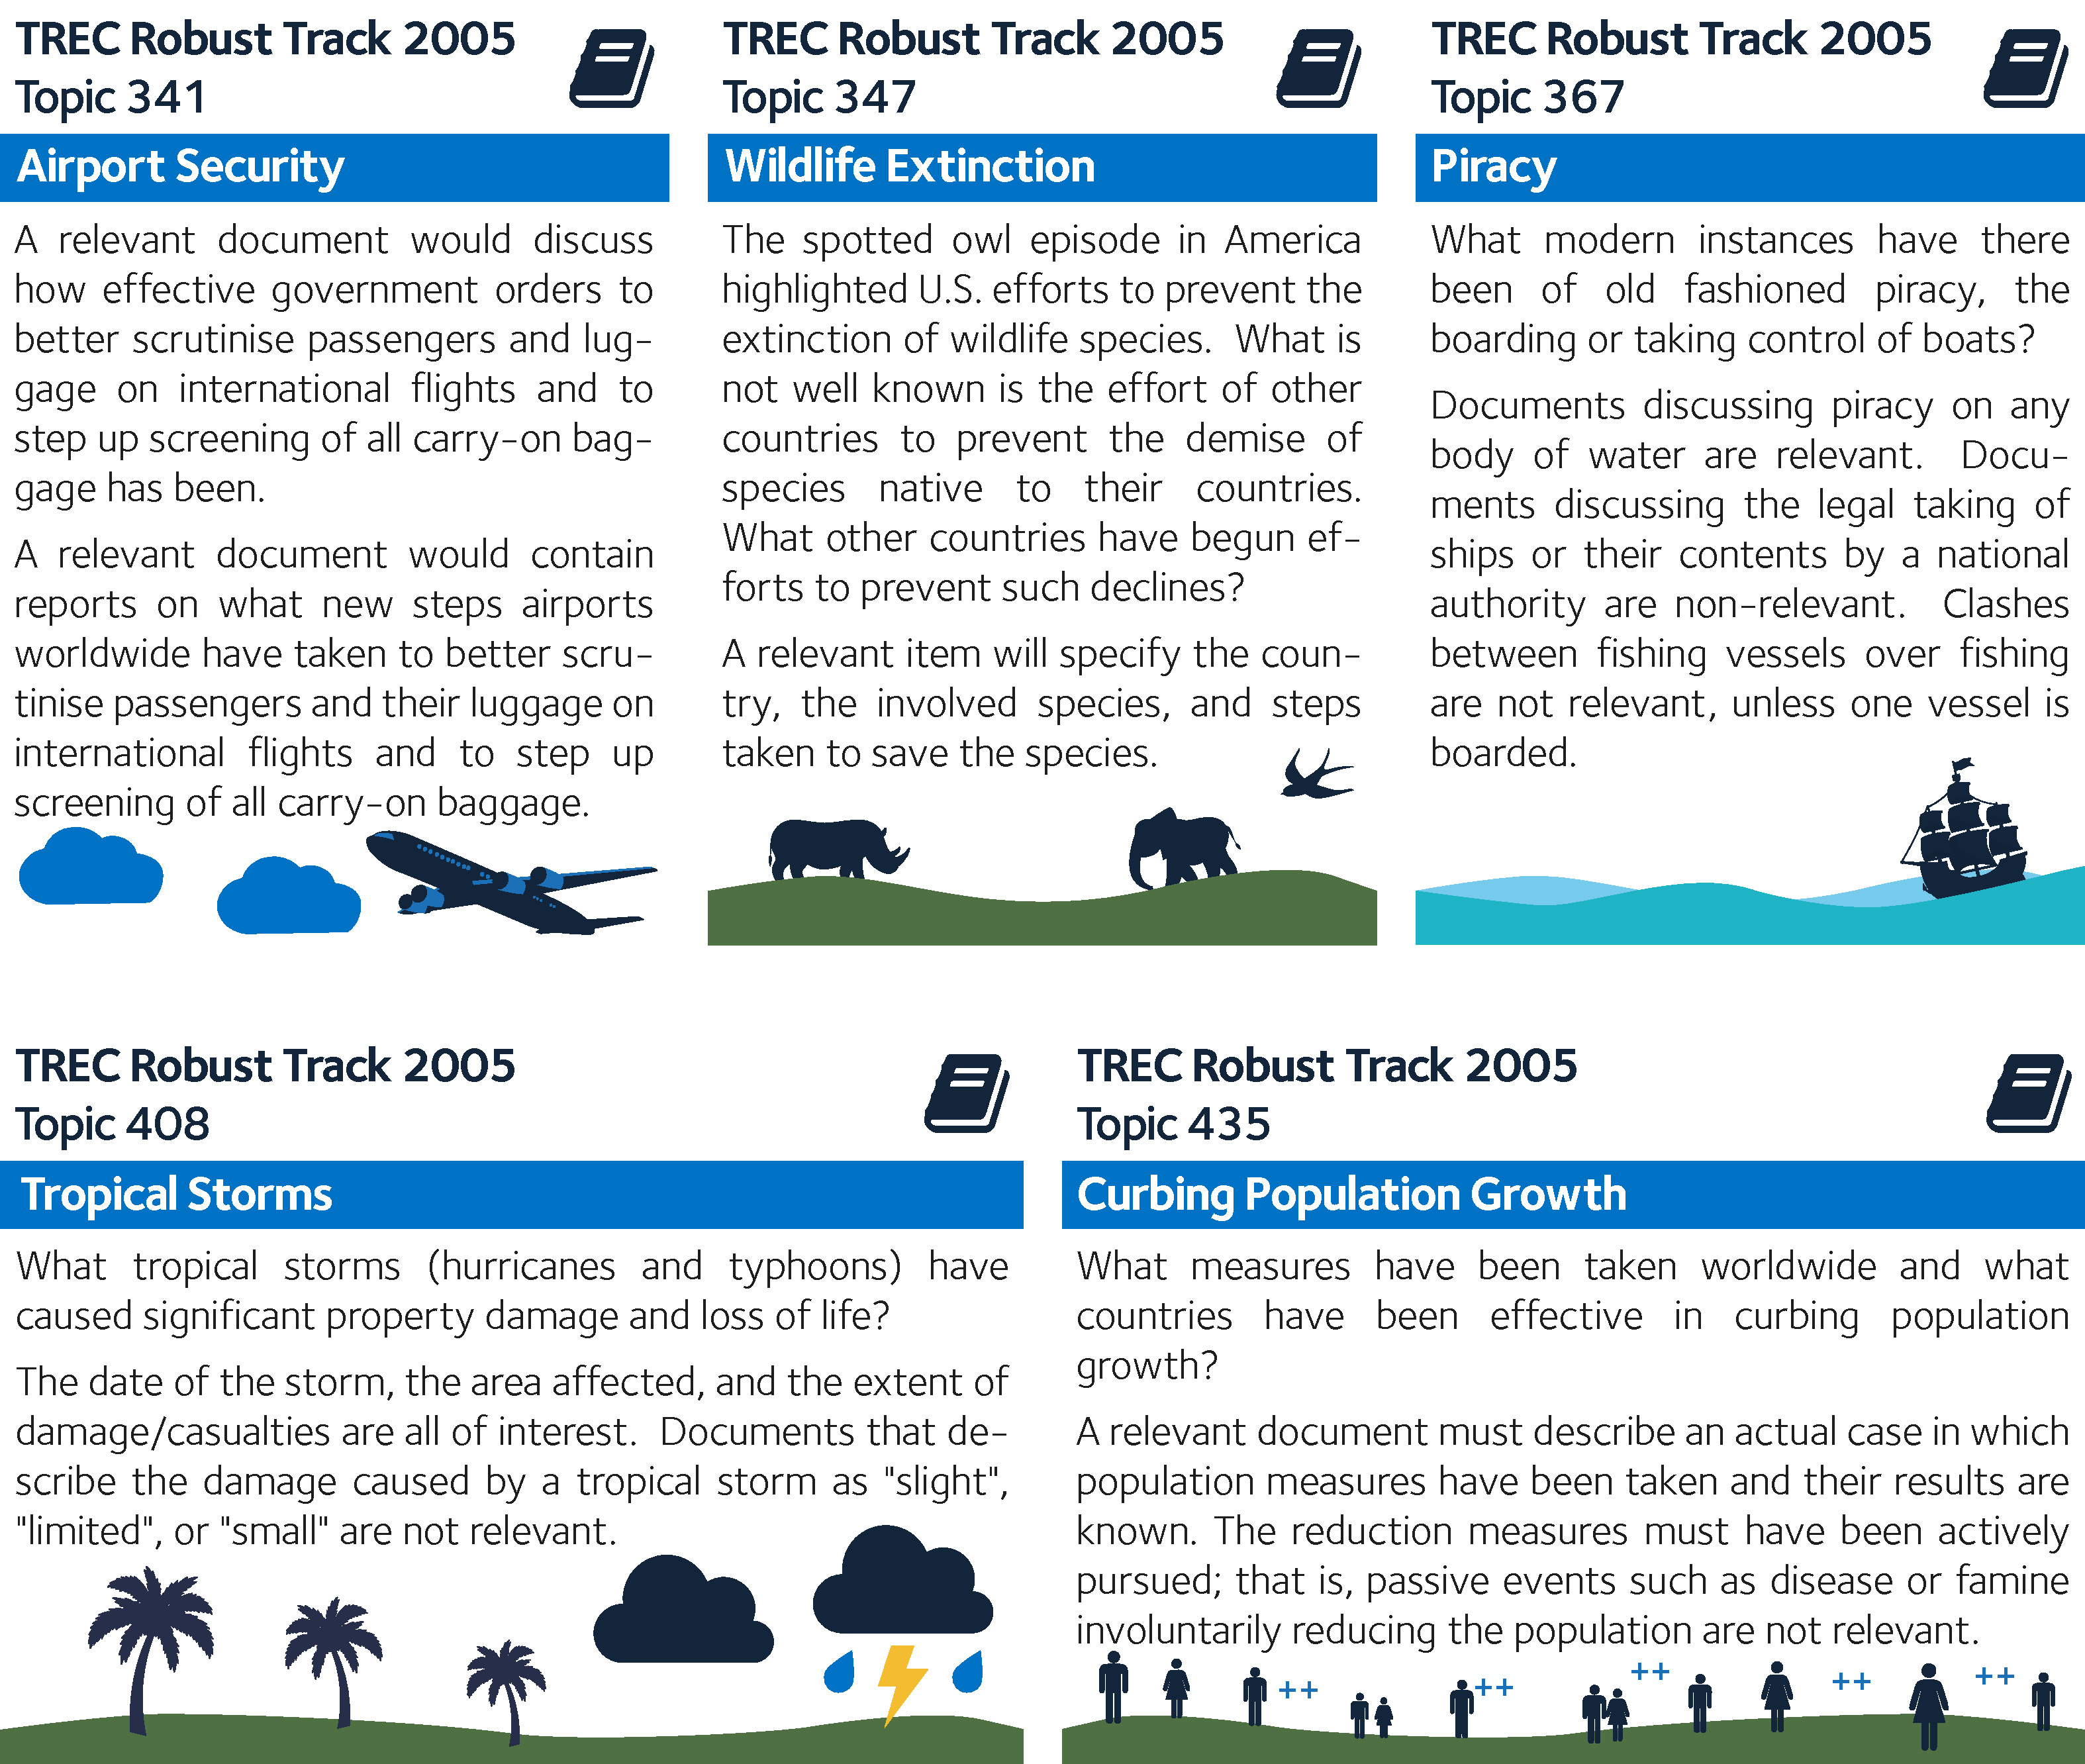
\includegraphics{figures/ch4-topics.pdf}}
    \caption[Examples of TREC Topics]{Three examples of \emph{TREC topic descriptions}, as outlined in Section~\ref{sec:csm:csm:flow}. Topics are extracted from the \emph{TREC 2005 Robust Track,} as outlined by~\cite{voorhees2006trec_robust}. Descriptions provide an explanation as to what constitutes a relevant (and often non-relevant) document.}
    \label{fig:topics}
\end{figure}

\begin{itemize}
    
    \item[]{\blueboxbold{Topic 341 – Airport Security} This topic considers relevant documents as those that discuss additional security measures that were taken by international airports around the world. Relevance is only denoted when a document discusses measures that go beyond the basic passenger and carry-on luggage screening. For example, AQUAINT document \texttt{NYT19980616.0123} discusses \emph{San Francisco International Airport's} attempts at introducing a \emph{robot sniffer,} attempting to look for nitroglycerine in luggage.}
    
    \item[]{\blueboxbold{Topic 347 – Wildlife Extinction} As the title of the topic suggests, this topic concerns wildlife extinction, and what efforts have been taken by countries other than the United States to counter the decline in endangered wildlife. Relevant documents explicitly mention the country, the species of animal, and the efforts the state or other governmental agency took to prevent decline in numbers. For example, document \texttt{XIE20000531.0205} discusses the breeding programme undertaken by China to bolster the number of Siberian Tigers in its jurisdiction.}
    
    \item[]{\blueboxbold{Topic 367 – Piracy} Instances of modern piracy are considered relevant to this topic -- not in the sense of software piracy, but the act of a water going vessel being boarded by individuals wishing to hijack it. Document \texttt{APW19980601.1065} provides an example of this -- the \emph{Petro Ranger}, a large fuel tanker, was boarded by pirates in 1998 in the South China Sea. To be relevant to the topic, the name of the vessel and the body of water it was hijacked on must be mentioned -- those discussing instances of when states intercepted vessels are not relevant.}
    
    \item[]{\blueboxbold{Topic 408 – Tropical Storms} Documents discussing major tropical storms are to be considered relevant, where the storm is reported to have caused significant damage and a large number of casualties. This is a particularly timely topic for the document corpus considered, as the 1998 hurricane season in the Caribbean has been reported to be one of the most costly -- both in terms of damage caused and lives lost -- in history.\footnote{This is reported by the US \emph{National Oceanic and Atmospheric Administration (NOAA),} as seen at \url{http://www.outlook.noaa.gov/98hurricanes/} -- last accessed May 15\textsuperscript{th}, 2018.} Document \texttt{APW19980921.1265} for example discusses the effects on Puerto Rico of Hurricane Georges in September 1998, leaving -- at the time of reporting -- three dead, many houses damaged, and thousands homeless.}
    
    \item[]{\blueboxbold{Topic 435 – Curbing Population Growth} The final topic considers efforts that have been made by countries around the world to control the ever increasing human population. Documents discussing this issue are only relevant to the topic if the results to a case have been made public, and a reduction in population has been actively pursued. The document must mention the country, the As such, events like famines are not relevant. A perhaps well known example of such a phenomenon is the one child policy that was pursued by China in the late 20\textsuperscript{th} century. Document \texttt{NYT19981031.0070} discusses the Chinese government's efforts to curb its expanding population at the time, with sexual education and heavy financial penalties for additional children. These efforts were shown to lead to a reduction in population, although whether this actually occurred is open to debate.}
    
\end{itemize}

For all user studies reported in this thesis, we selected topic \blueboxbold{367} as a \emph{practice topic,} permitting the participating subjects to familiarise themselves with the experimental system used. As such, we do not report any results from interactions that took place with this topic -- comparisons between simulated and actual searcher behaviours are also omitted. 

All queries submitted during experiments were also handled with the \emph{Whoosh~\gls{acr:ir} Toolkit}.\footnote{\emph{Whoosh} can be freely acquired using the \texttt{pip} \emph{Python} package manager -- documentation for Whoosh is available online at \url{http://whoosh.readthedocs.io/en/latest/intro.html} (last accessed May 15\textsuperscript{th}, 2018). The corpus was indexed with Whoosh \texttt{2.7.4}.} Using the toolkit, we indexed the AQUAINT document collection, applying Porter stemming. Stopwords -- from Fox's classical stopword list -- were also removed (refer to Section~\ref{sec:ir_background:basics:indexing} for more information on the indexing process). For this index, we also removed documents with \todo{duplicate titles}. This is an issue, especially with documents originating from a newswire. A document discussing an ongoing event may be continually revised as new information arises, leading to multiple revisions. \todo{For documents with duplicate titles, we retained the document with the latest timestamp.}

With an index weighing in at 800MB, consisting of $128,894$ documents. \todo{What else did we do to reduce this number?} We could then issue queries against the index. All ranked results from queries were computed with the BM25 algorithm, where $\beta=0.75$. Terms in the queries issues were implicitly \texttt{AND}ed together to restrict the set of retrieved documents to those that only contained all of the query terms. This was chosen to reduce the size of the returned set -- most search systems employ such an implicit approach.

\section{User Study Framework}\label{sec:method:user_study}
Using the document collection, topics and search engine outlined above, we now move onto discussing the common methodology used for the two user studies. These are detailed in Chapters~\ref{chap:snippets} and~\ref{chap:diversity}. While intricate details of each study's methodology do indeed vary, there are nevertheless common components between both that we discuss here. As a reminder, the two studies examine how a searcher's behaviours, performance and perceived user experience varies when:

\begin{itemize}
    \item{the length (and thus quality) of snippets presented in result summaries are varied (Chapter~\ref{chap:snippets}, conducted between July and August, 2016); and}
    
    \item{the overall search goal (time constraints vs. relevancy accruement) and task goal (ad-hoc vs. diversified results) are changed (Chapter~\ref{chap:diversity}, conducted in January, 2018).}
\end{itemize}

Specifically, the methodology used for these studies allowed us to determine how the stopping behaviour of a searcher varies when these conditions are varied. We discuss the specific interfaces and conditions that we trialled in subsequent chapters of this thesis.

Both user studies were undertaken using a custom built experimental framework called \blueboxbold{TREConomics}.\footnote{\treconomics~can be found online at \url{https://github.com/leifos/treconomics} -- \urlaccessed{2018-05-15}.} The pure-\emph{Python} framework has been developed over a number of years, and allows straightforward deployment of various~\gls{acr:iir}-based studies. It has been successfully deployed in a number of prior works, including those by~\cite{azzopardi2013query_cost},~\cite{maxwell2014temporal_delays} and~\cite{kelly2015serp_size}.

\subsection{Experimental Details and Flow}\label{sec:csm:methodology:user:flow}
Subjects who participated in the two different user studies spent approximately 45-50 minutes of their time performing the requested tasks (including completion of all surveys, as discussed below). Both experiments followed a similar structure, where subjects would complete a number of surveys before beginning a search task, and completing a further survey upon completion of the task. These surveys, as discussed in Section~\ref{sec:csm:methodology:extracting:user}, permitted us to gather information about the subjects' perceived experiences when trialling the various interfaces and conditions.

The basic structure of both user studies was as follows. To reiterate, this is a general structure -- refer to the relevant chapter detailing each of the two studies for more detailed information about the setup of the relevant study.

\begin{itemize}
    \item{Subjects began by reading the experiment briefing sheet, before agreeing to continue.}
    \item{A demographics survey was then completed.}
    \item{Subjects then attempted the \emph{practice task,} using the practice topic as highlighted in Section~\ref{sec:csm:methodology:collection}. This allowed subjects to familiarise themselves with the system and its interface (as discussed in Section~\ref{sec:csm:methodology:user:interface}).}
    \item{Subjects would then complete the various search tasks set out for them. Each task consisted of three steps:}
    
    \begin{itemize}
        \item{a pre-task survey, capturing a subject's prior knowledge about the topic;}
        \item{the search task itself; and}
        \item{a post-task survey, capturing the subject's experiences regarding searching for information about the topic.}
    \end{itemize}
    
    \item{Upon completion of each search task, subjects would then complete a post-experiment survey, asking general questions about their experience across all the different tasks.}
    \item{Finally, upon completion, subjects would be presented with a results screen, providing a summary of their performance. Performance for each subject was presented on a per-task basis. At this point, the experiment concluded.}
\end{itemize}

Given the document collection used, search tasks were grounded with subjects instructed to imagine that they were newspaper reporters, and were required to gather documents to write stores about the given topics. Although goals stated to subjects varied (refer to Chapters~\ref{chap:snippets} and~\ref{chap:diversity} for further information), subjects were asked to \emph{identify} a number of documents that they thought were relevant to the given topic. Further explanation on this is provided in Section~\ref{sec:csm:methodology:user:interface}.

Subjects also undertook a total of four search tasks in which interactions and experiences were captured. Including the practice task at the beginning of each experiment, this took the total number of search tasks per subject up to five. Following a \blueboxbold{within-subjects study design}, the four search tasks -- each using a different topic as described in Section~\ref{sec:csm:methodology:collection} -- permitted us to trial each different experimental condition/interface. The topics and tasks were assigned to subjects using a Latin-square rotation to minimise topic ordering effects. Our primary motivation for selecting a within-subjects design was that of data acquisition -- a within-subjects design permits a greater volume of data to be captured from a study following a between-subjects design.

\subsection{Experimental Search Interface}\label{sec:csm:methodology:user:interface}
As both experiments used the \treconomics~framework, a similar search interface was used for both. However, slight modifications were employed for the goal-based study interface, as detailed in Section~\ref{chap:diversity}. The interface would be familiar to anyone who has used a web-based retrieval system, and thus the learning curve for using the interface would most likely be low. Upon commencement of the experiment, the interface would launch in a fixed-size popup window (refer to Section~\ref{sec:csm:methodology:user:crowdsourcing:technical}) of the web browser being used.

Note that here we only discuss the experimental search interface -- as per the section title. To be more specific, this is the interface that subjects used when undertaking the various search tasks we asked them to perform. The interface consists of three main views, the two most important being shown in Figure~\ref{fig:interfaces}. The views were:

\begin{itemize}
    \item{the~\glsfirst{acr:serp}, presenting the query box and results for an issued query;}
    \item{the \emph{document view,} providing the source text of an article; and}
    \item{the \emph{saved documents list,} providing a list of the documents that subjects had identified as relevant.}
\end{itemize}

In addition to the three views above, we also provided a \emph{topic view,} which, when requested, would open a further popup window that contained a description of the topic. This was purely to serve as a reminder, as subjects were provided the topic description in full before the search task began. Common to all views was the inclusion of the blue navigation bar at the top of the popup window. As we discuss further in Section~\ref{sec:csm:methodology:user:crowdsourcing:technical}, this bar was included to provide a series of different navigational links, such as, when on the document view page, a link to return to the originating~\gls{acr:serp}. Where applicable, we also provided a link for the subject to end the search task, if he or she felt that they had satisfied the criteria for the task.

\begin{figure}[t!]
    \centering
    \resizebox{1\hsize}{!}{
    
\includegraphics[width=1\textwidth]{figures/ch6-interfaces.png}}
    \caption[Example screenshots of the experimental interfaces]{Example screenshots of the basic search interface used as part of \treconomics. On the left is a screenshot of typical experimental~\gls{acr:serp} for the query \texttt{wildlife extinction}. The right shows the document view, showing the option for subjects to \texttt{Save} a document that they consider relevant to the given topic.}
    \label{fig:interfaces}
\end{figure}

\subsubsection{The Search Engine Results Page}
As can be observed from the left screenshot in Figure~\ref{fig:interfaces}, the~\gls{acr:serp} does not look all that different from a~\gls{acr:serp} on a contemporary web search engine -- sans right rail components, as we discussed previously in Section~\ref{sec:ir_background:basics}. The experimental~\gls{acr:serp} provides at the top the \emph{query box,} allowing subjects to enter their query term(s), and a button to submit their query. The \texttt{ENTER} key could also be used to submit a query.

Once submitted, results are displayed underneath the query box. The issued query is provided, along with an approximation of how many pages of results are provided to the searcher for the given query. This hints that pagination is utilised -- with 10 results per page shown. At the bottom of each~\gls{acr:serp} are links that allow the searcher to move to the next page, and vice versa.

Result summaries are shown in the accepted way -- the title, the source, and any snippet text are all provided. Given that the experiment is based upon news search, the source is the name of the newswire from which the document originates. The title was also hyperlinked -- when a subject clicked on the link, he or she would then be taken to the document view (discussed below), displaying the associated document in its entirety. Standard hyperlink colours were employed -- blue for unvisited, and purple for visited.

\subsubsection{The Document View}
The right screenshot in Figure~\ref{fig:interfaces} illustrates the document view. Particularly unexciting, the view provides the title, the document source (newswire), the date at which the document was created, and the full text of said document. On the right rail of the page, subjects were provided with two buttons -- one to return them to the originating~\gls{acr:serp}, or another to \emph{save} the document. The act of saving a document is a crucial component to both studies we discuss in this thesis. It provided us with a mechanism to determine what documents subjects thought were relevant to the given topics. Thus, this mechanism, for instance, also provided us with a means to calculate a subject's performance. Once clicked, the document was appended to a list of previously saved documents that subjects could also view.

\subsubsection{The Saved Documents View}
The third key view, as mentioned above, allowed subjects to view a list of documents that they had previously saved as relevant to the given topic. This list of documents also provided buttons, allowing subjects to change their decisions as to what constituted as a relevant document. We provided this functionality as~\gls{acr:iir} is inherently an interactive process -- a searcher \emph{learns} and develops their mental model of the given information need as more information is presented to them~\citep{ingwersen2005theturn}.

\subsection{Capturing Interactions and Survey Responses}\label{sec:csm:methodology:user:capturing}
In addition to the front-end interface provided to the subjects of each experiment, the \treconomics~framework also provided extensive logging capabilities to capture a variety of different events triggered by subjects as they performed the search tasks. This resulted in an generation of an experiment \emph{log file,} capturing the date, time, user and topic for each event that was logged. Figure~\ref{fig:log} provides an anonymised excerpt from the interaction log of the snippets user study, as discussed in Chapter~\ref{chap:snippets}. The figure illustrates the different actions that were logged from when a searcher begins interactions with the query box (\texttt{QUERY\_FOCUS}), to issuing a query (\texttt{QUERY\_ISSUED}, complete with the terms of the query), to clicking a document (\texttt{DOC\_CLICKED}), and, finally, to saving the document (or considering it relevant to the given topic, \texttt{DOC\_MARKED\_RELEVANT}). A detailed discussion of the different behavioural measures that we examined from the interaction log are detailed in Section~\ref{sec:csm:methodology:extracting}.

\begin{figure}[t!]
    \centering
    \resizebox{1\hsize}{!}{
    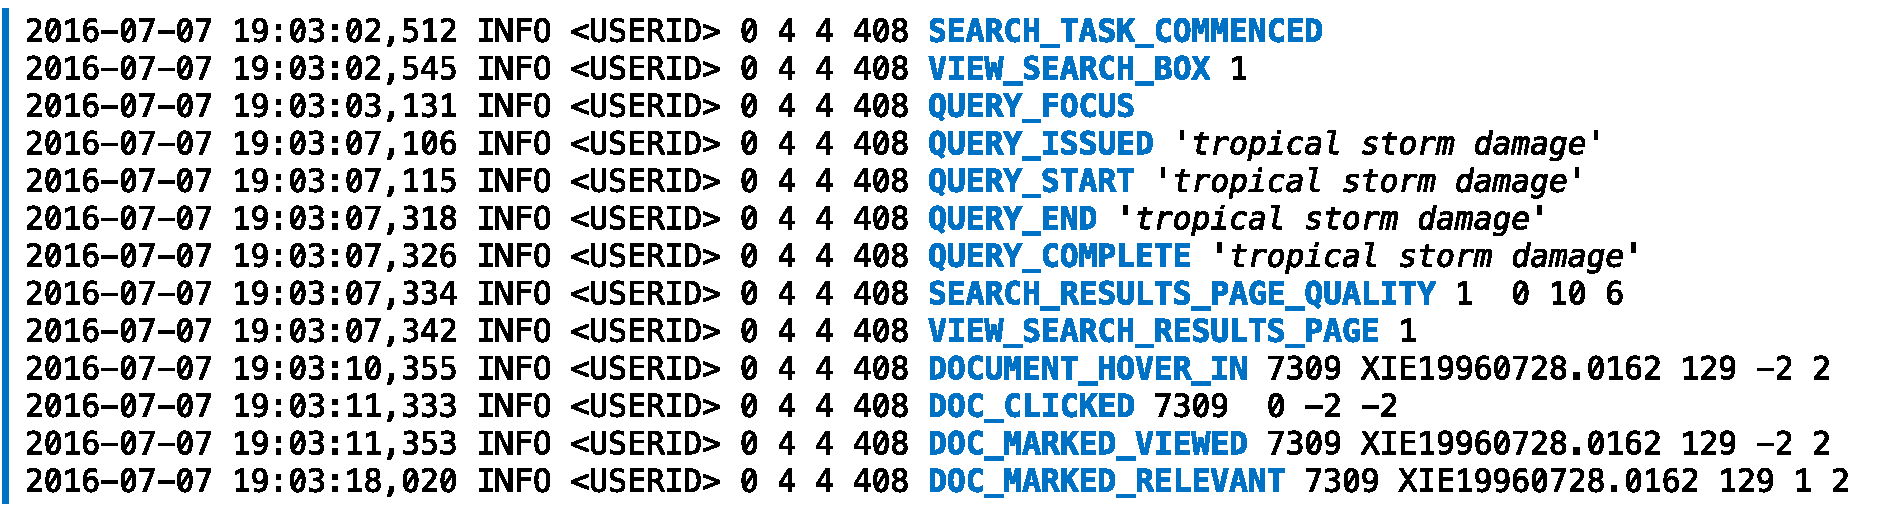
\includegraphics{figures/ch6-log.pdf}}
    \caption[Experiment log file excerpt]{An excerpt from the snippets user study, as detailed in Chapter~\ref{chap:snippets}. This example provides a sequence of interactions that were logged by the\treconomics~framework.}
    \label{fig:log}
\end{figure}

In addition to the interaction log, the \treconomics~framework also saved the responses from surveys as filled in by the subjects of each study. These were saved to a separate~\gls{acr:rdbms}, with a number of scripts subsequently created to extract and analyse the saved responses.

\subsection{Crowdsourcing Considerations}\label{sec:csm:methodology:user:crowdsourcing}
An important factor in planning any user study is the economics of collecting input from subjects. \emph{Where do the subjects come from? How do we recruit them?} A traditional, lab-based study as discussed in Section~\ref{sec:ir_background:user} typically involves a significant investment in time and monetary cost from the researchers conducting the experiment~\citep{spool2001testing}. For both user studies previously detailed, we employed a \emph{crowdsourced} approach to our experimentation. Crowdsourcing is the practice of obtaining input into a task by enlisting the services of a number of people, recruited over the Internet.

As highlighted by Zuccon et al.~\cite{zuccon2013crowdsourcing_comparisons}, crowdsourcing provides an alternative means for capturing user interactions and search behaviours. Greater volumes of data can be obtained from more heterogeneous workers at a lower cost -- all within a shorter timeframe. Of course, pitfalls of a crowdsourced approach include the possibility of workers completing tasks as efficiently as possible, or submitting their tasks without performing the requested operations~\citep{feild2010turkers}.

Despite these issues, it has been shown that there is little difference in the quality between crowdsourced and lab-based studies~\cite{zuccon2013crowdsourcing_comparisons}. Nevertheless, quality control is a major component of a well-executed crowdsourced experiment~\cite{bota2016information_cards}. Employing crowdsourcing for our two user studies, we detail in the remainder of this section the precautions that were taken during, discussing both the requirements for the subjects and their technical setup -- as well as a discussion of the crowdsourcing platform used.

\subsubsection{Platform Details}
Both studies were run over the \emph{Amazon Mechanical Turk (MTurk)} platform. Workers\footnote{In this section, a \emph{worker} refers to an individual undertaking the experiment on the MTurk platform. This term is considered interchangeable with a \emph{subject.}} from the platform each performed a single task (or, to use MTurk language, a \emph{Human Intelligence Task (HIT)}), with a single HIT corresponding to the entire experiment. This is in contrast to many HITs, where workers would typically undertake small, typically decision-based, transactions (for an example of such a study where this took place, refer to~\cite{bota2016information_cards}).

\subsubsection{Subject Requirements}
Due to the expected length that workers would take to complete the two studies\footnote{Note that two different sets of workers were used -- the studies were run at different times.}, workers who completed the study in full were reimbursed for their time with US\$9 -- greater than the hourly minimum wage set by the US federal government. Workers interested in undertaking each of the two studies were required to meet a certain minimum set of criteria to be eligible to participate. We required that workers were:

\begin{itemize}
    \item[\emph{(i)}]{from the United States;}
    \item[\emph{(ii)}]{native English speakers;}
    \item[\emph{(iii)}]{possessed a HIT acceptance rate of at least 95\%; and}
    \item[\emph{(iv)}]{had at least had 1000 prior HITs approved.}
\end{itemize}

Requiring \emph{(iii)} and \emph{(iv)} reduced the likelihood of recruiting workers who would not complete the study in a satisfactory manner. Recruits were forewarned about the length of the HIT, providing them with a chance to abandon the experiment if they felt the expected time was too long.

\subsubsection{Technical Requirements}\label{sec:csm:methodology:user:crowdsourcing:technical}
Given worker limitations, we also enforced a number of technical constraints. Workers attempting each experiment were required to have a sufficiently large computer screen to display the experimental interface without having to resort to excessive scrolling, and ensured a consistent number of result summaries would be present on different worker's screens. As such, we imposed a minimum display resolution of $1024x768$ for both studies. Conducted through a web browser, we wanted to ensure that only the controls provided by the experimental apparatus were used, meaning that the popup window that we highlighted in Section~\ref{sec:csm:methodology:user:interface} had all other browser controls disabled to the best of our ability (i.e. browser history navigation, etc.). The experimental system was tested on several major web browsers, across different operating systems. This gave us confidence that a similar experience would be had across different system configurations.

\section{Extracting User Study Data}\label{sec:csm:methodology:extracting}
As discussed in Section~\ref{sec:csm:methodology:user:capturing}, the \treconomics~framework provided the necessary infrastructure for us to log the various interactions and capture survey responses from each individual subject across the two user studies trialled. In this section, we provide details on the different aspects that we subsequently used to evaluate searcher behaviours, performance and user experience. Figure~\ref{fig:evaluation_methodology} provides a graphical illustration of how we split the various aspects we consider into four distinct categories.

The first three categories can be extracted directly from the interaction log that recorded different interactions by each subject as they progressed through the experiment. The categories we considered are listed below.

\begin{itemize}
    
    \item[]{\blueboxbold{Behavioural Measures} capture the broad interactions that take place, such as the number of documents that a searcher examined in detail.}
    \item[]{\blueboxbold{Performance} measures could be extrapolated, with aid of~\gls{acr:trec} QREL relevance judgements, to ascertain the performance of subjects.}
    \item[]{\blueboxbold{Time-Based} measures can also be derived from directly examining the interaction log, measuring the time spent between different logged interactions.}
    
\end{itemize}

In addition to these categories, we also observed a number of \blueboxbold{user experience} measures that are derived from a series of surveys that subjects were presented with as they were walked through the experimental process. In particular, as highlighted in Section~\ref{sec:csm:methodology:user:flow}, surveys were presented to subjects at a number of different stages throughout the experiment. In conjunction with the three log-based categories defined above, the user experience measures could be used to complement the empirical evidence to see whether the interactions of subjects actually correlated with their perceived experiences.

In all, the interactions -- including aspects such as clicks, and time-based measures, were used as a \emph{grounding} for our subsequent user simulations. These are discussed in Section~\ref{chap:csm:method:simulation} and derived for each experimental condition and interface trialled.

\begin{figure}[t!]
    \centering
    \resizebox{1\hsize}{!}{
    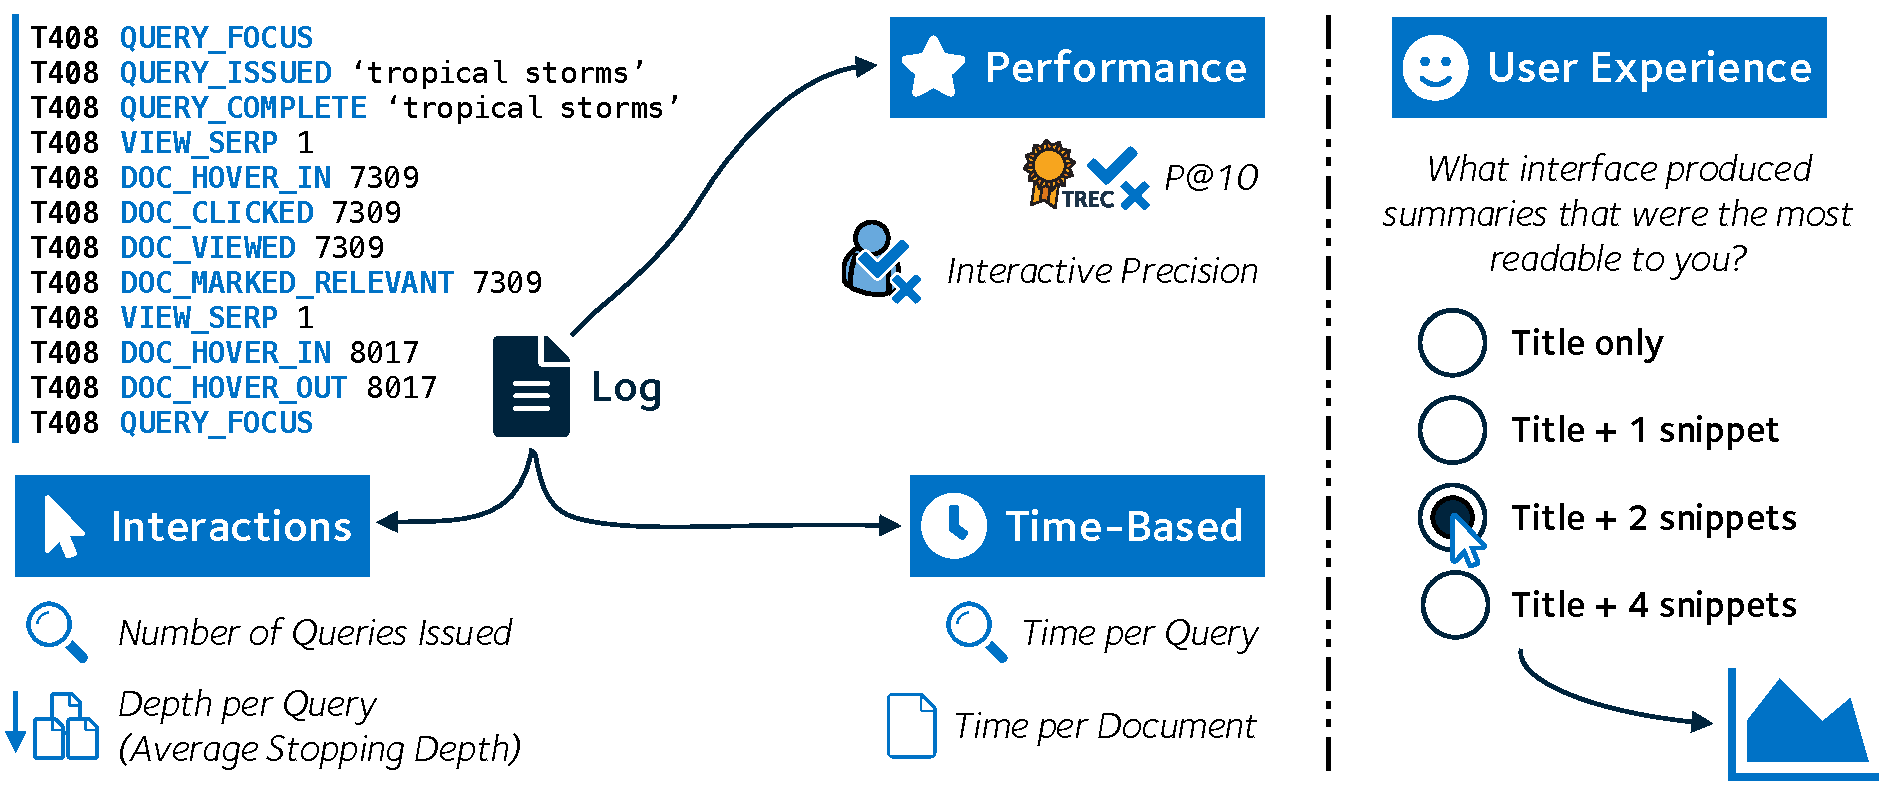
\includegraphics{figures/ch4-evaluation.pdf}}
    \caption[Examples of Evaluation Measures]{An illustration of the different types of measures that are captured, and from what sources. Interaction, time-based and performance measures are derived from the user study experiment log (with~\gls{acr:trec} QRELs used in conjunction with the interaction log to compute a subject's performance). User experience metrics are collated from a number of different surveys. Refer to Section~\ref{sec:csm:methodology:extracting} for more information.}
    \label{fig:evaluation_methodology}
\end{figure}

\subsection{Behavioural Measures}
Recorded solely from interaction log data, the basic interactions covered a large proportion of the aspects we considered in our analyses. They key behavioural measures we examined were:

\begin{itemize}
    \item{the number of \blueboxbold{queries issued};}
    \item{the number of \blueboxbold{documents viewed};}
    \item{the number of \blueboxbold{\glsplural{acr:serp} viewed}; and}
    \item{the \blueboxbold{depths} to which subjects clicked on (and hovered over), regarding the result summaries presented on the~\glsplural{acr:serp}.}
\end{itemize}

From these measures, we could then ascertain whether searcher behaviour varied when a certain condition or interface was changed -- allowing us to address questions such as \emph{whether snippet length affects the depth to which searchers examine content?} To compute depths, click and hover depths were used -- we however only report click depths in subsequent contributory chapters. The reasoning for this is discussed in Section~\ref{sec:csm:methodology:extracting:time} below. These measures were observed over each query issued by subjects.

% -- we could then take an average for each subject. We could go even further, too -- averaging over each topic, interface or condition as required to observe any notable trends in behavioural changes.

\subsection{Time-Based Measures}\label{sec:csm:methodology:extracting:time}
As discussed in Section~\ref{sec:csm:methodology:user:capturing} -- and also illustrated in Figure~\ref{fig:log} on page~\pageref{fig:log}, each logged interaction was saved with a timestamp which allowed us to determine when each event occurred.\footnote{Timestamps were saved to the nearest thousandth of a second, as per the specification of the standard Python logging framework -- refer to \url{https://docs.python.org/2/howto/logging-cookbook.html} \urlaccessed{2018-05-29} for an example of the framework in action.}. With these timestamps, we could then measure the time between two associated events, thus yielding the time taken to perform a given activity. We considered five key time-based measures across both user studies, namely:

\begin{itemize}
    \item{the time spent \blueboxbold{issuing queries};}
    \item{the time spent examining the \blueboxbold{content on~\glsplural{acr:serp}};}
    \item{the time spent examining \blueboxbold{individual result summaries};}
    \item{the time spent examining \blueboxbold{documents}; and, of course}
    \item{the summation of all of the above to yield the \blueboxbold{total session time}.}
\end{itemize}

It should be noted that in this thesis, \blueboxbold{we report all durations in seconds}. Event durations from the interaction log could be calculated in a relatively straightforward fashion. For example, the duration between the \texttt{QUERY\_FOCUS} to \texttt{QUERY\_ISSUED} events yielded the subject's query time. We of course acknowledge that in all likelihood, subjects may have considered what query to issue before focusing on the query box. However, we did not have the tools at our disposal to measure this. 

One further point worthy of note was how we computed the time spent examining each result summary. The per result summary time was approximated by taking the total time spent on a given~\gls{acr:serp}, and dividing that value by the click depth that was reached on that~\gls{acr:serp}. This was originally computed by summing up the time spent hovering over results with the subject's mouse cursor, as this was shown in prior studies to correlate strongly with the user's gaze on the screen~\citep{chen2001mouse_cursor, smucker2014judging_relevance_movements}. However, issues with network latency meant that several of the hover events were logged in the incorrect order, making such an approach unviable. Using the click depth and total~\gls{acr:serp} time provided us with an approximation with which to work with. However, the approximation also makes an assumption that subjects examined each result summary on a~\gls{acr:serp}, up until a particular depth, for an equal period of time. This was sufficient for the work in our study to ascertain whether or not a variation in the task goal or presentation of results affected search depths.

\subsection{Performance Measures}
As previously discussed, we were also able to extract a number of different performance measures from the interaction logs, too. Using the raw data from the logs, we could then, in conjunction with our set of~\gls{acr:trec} QRELs, compute a number of performances measures.\footnote{Some measures were computed with the \texttt{trec\_eval} evaluation tool, discussed in Section~\ref{sec:ir_background:basics:cranfield:trec}.} Key performance measures that we captured included:

\begin{itemize}
    \item{the \blueboxbold{overall performance of queries}, measured with \blueboxbold{P@10}; and}
    \item{\blueboxbold{interactive precision and recall} (as discussed in Section~\ref{sec:ir_background:user:evaluation:interactive_pr}), including:}
    
    \begin{itemize}
        \item{the number of documents saved (identified as relevant); and}
        \item{the number of those documents that were~\gls{acr:trec} relevant (and vice-versa).}
    \end{itemize}
\end{itemize}

\blueboxheader{Grounding Subsequent Experiments} With behavioural measures and time-based measures in particular, these could be then used to \emph{ground} subsequent experiments. Refer to Section~\ref{chap:csm:method:simulation:grounding} for further information on how this was achieved. The above measures are however sufficient for analysing how searcher behaviour changed under different contexts.

\subsection{Demographics and User Experience Surveys}\label{sec:csm:methodology:extracting:user}
A number of surveys, as discussed in Section~\ref{sec:csm:methodology:user:capturing}, were also filled out by subjects capturing a variety of information about their search experiences. While there are similarities between what is asked (refer to Chapters~\ref{chap:snippets} and~\ref{chap:diversity} for further details), we in this section provide a high-level overview of the different surveys, before examining questions that were common between the two. We break these overviews into three sections, in the order of the experimental flow detailed in Section~\ref{sec:csm:methodology:user:flow} -- demographics, pre- and post-task surveys, and post-experiment surveys.

\subsubsection{Demographics}
Details in keeping with general demographics were attained about the different subjects from this survey. These included the subject's age, gender and occupation. We also queried the subject on their highest level of professional qualification (e.g. high school, Honours, MSc or PhD). A number of questions were also asked about their perceived proficiency and approach to searching for information on the~\gls{acr:www}. Questions included how often they searched for information, what pointing device they were using (i.e. mouse, trackpad), and their preferred web search engine. Finally, given that both experiments considered news search, we asked how often the subjects searched for news articles online.

\subsubsection{Pre-Task}
Between both user studies, we asked the same questions within the pre-task survey. Subjects were provided with a short description of their search task and a topic description, providing their information need for said task. After examining the topic description, subjects were then queried on the following:

\begin{itemize}
    \item{how well they knew about the topic prior to this study;}
    \item{how relevant the topic was to their life;}
    \item{how interested they were to learn more about the topic;}
    \item{whether they had searched for information related to the topic before; and}
    \item{how difficult they felt it would be to search for information on the topic before commencing.}
\end{itemize}

Responses were provided on a five-point scale, providing the option for neutrality between the two extremes -- extremes being \emph{nothing/not at all/very difficult} to \emph{lots/very much/very easy.} Responses to these questions helped us gauge the perceived difficulty of the task, and ascertain how much background knowledge could potentially affect results.

\subsubsection{Post-Task and Post-Experiment}
Post-task and post-experiment surveys were unique to each of the two user studies. Chapters~\ref{chap:snippets} and~\ref{chap:diversity} provide further information on what questions were asked. However, the post-task surveys focused on how well the subjects thought they (and the retrieval system, under the given condition and/or interface) performed during the search task. Post-task surveys considered the experiment as a whole, asking a range of questions about what condition and/or interface the subjects preferred, or performed more to their liking, for example.

\section{Simulating Searcher Behaviours}\label{chap:csm:method:simulation}
Simulation as defined earlier is a good means for experimentation.
Low cost, always use the same users, no issue of learning bias, etc.

EXPLORE how people's behaviours change

- set up the probabilities
- instantiate the components

- pick a topic set
- pick a corpus
- basic structure of the methodology from previous papers

Probabilities - From this raw data, we could then produce summaries of a search session, producing summarising measures such as the number of documents examined by searchers per query that they issued. We could also calculate from the log data probabilities of interaction, including a given subject’s probability of clicking a result sum- mary link, given that it was TREC relevant (P(C|R)) or TREC non- relevant (P (C |N )) – or the probability of marking a document that was clicked, given it was either TREC relevant (P(M|R)) or TREC non-relevant (P (M |N )). Actions such as hover depth over result summaries were inferred from the movement of the mouse cursor, which in prior studies has been shown to correlate strongly with the user’s gaze on the screen [7, 44].

\subsection{Grounding the Simulations}\label{chap:csm:method:simulation:grounding}

\subsection{Instantiating the Simulations}

\subsection{Performance Runs}

\subsection{Comparison Runs}

\section{Evaluation of Simulations}\label{chap:csm:method:evaluation}
- how do we evaluate how good the system performs?
- how do we work out which one approximates best? on average.

\subsection{Determining Simulated User Performance}

\subsection{Comparing Simulated and Real-World Subjects}

\section{Chapter Summary}